% % % % % % % % % % % % % % % % % % % % % % % % % % %
% IS&T Template
% ECE5110 Unit 03 Article
% Three-Point Finite-Difference Differentiation and
% Gravitational Acceleration Estimation from Free-Fall Data
% % % % % % % % % % % % % % % % % % % % % % % % % % %

%%%%%%%%%%%%%%%%%%%%%%%%%%%%%%%%%%
% Document class
%%%%%%%%%%%%%%%%%%%%%%%%%%%%%%%%%%
\documentclass[letterpaper,twocolumn,fleqn]{article}

%%%%%%%%%%%%%%%%%%%%%%%%%%%%%%%%%%
% Packages
%%%%%%%%%%%%%%%%%%%%%%%%%%%%%%%%%%
\usepackage{ist}
\usepackage{amsmath}
\usepackage{amssymb}
\usepackage{siunitx}
\usepackage{physics}
\AtBeginDocument{\RenewCommandCopy\qty\SI}
\ExplSyntaxOn
\msg_redirect_name:nnn { siunitx } { physics-pkg } { none }
\ExplSyntaxOff

\pagestyle{empty}

%%%%%%%%%%%%%%%%%%%%%%%%%%%%%%%%%%
% Title and Authors
%%%%%%%%%%%%%%%%%%%%%%%%%%%%%%%%%%
\title{Three-Point Differentiation and Composite Integration: Unit 03 Numerical Validation on Analytic and Experimental Data}
\author{
Carson Quesada; California Polytechnic University Pomona; Pomona, California \\
Ishmael Taleo; California Polytechnic University Pomona; Pomona, California \\
Juan Ortiz; California Polytechnic University Pomona; Pomona, California \\
Michael Lanfranchi; California Polytechnic University Pomona; Pomona, California \\
Rushi Sharma; California Polytechnic University Pomona; Pomona, California \\
Timothy Jung; California Polytechnic University Pomona; Pomona, California
}
\date{}

%%%%%%%%%%%%%%%%%%%%%%%%%%%%%%%%%%
% Begin document
%%%%%%%%%%%%%%%%%%%%%%%%%%%%%%%%%%
\begin{document}
\maketitle
\thispagestyle{empty}

%%%%%%%%%%%%%%%%%%%%%%%%%%%%%%%%%%
% Abstract
%%%%%%%%%%%%%%%%%%%%%%%%%%%%%%%%%%
\begin{abstract}
Unit 03 numerical workflows were implemented and validated for both differentiation and integration. Three-point finite-difference formulas---central, forward, and backward---were tested on three analytic derivatives: $\sin(x)$ at $x=\pi/4$, $e^{x}$ at $x=0.3$, and $x^{3}-2x^{2}+x-5$ at $x=1.2$. All nine method-function combinations achieved absolute errors below $\num{1.5e-10}$. Composite trapezoidal and composite Simpson integration were then evaluated on
\[
\int_{0}^{1} \frac{4}{1+x^2}\,dx=\pi,
\]
using $n=4$ to $256$ subintervals. Trapezoidal converged at observed order $1.99999$ with finest absolute error $\num{2.543e-6}$, while Simpson reached near machine precision at the finest mesh and passed all prescribed tolerances. Finally, a free-fall dataset was fit with a quadratic interpolant and numerically differentiated twice to estimate gravity, yielding $|\hat{g}|=\qty{9.6904}{m/s^2}$ with magnitude error $\qty{0.1196}{m/s^2}$ versus $\qty{9.81}{m/s^2}$.
\end{abstract}

%%%%%%%%%%%%%%%%%%%%%%%%%%%%%%%%%%
% Introduction
%%%%%%%%%%%%%%%%%%%%%%%%%%%%%%%%%%
\section{Introduction}
\label{sec:intro}
Numerical differentiation and numerical integration are core operators in scientific computing. In many engineering workflows, derivatives and integrals must be estimated from discrete samples rather than symbolic expressions. Reliable finite-difference and quadrature methods therefore provide the bridge from sampled data to physical inference.

Three-point stencils offer second-order derivative accuracy, $O(h^{2})$, with compact local evaluations. Composite trapezoidal and Simpson rules offer globally second-order and fourth-order integral convergence, respectively, on smooth integrands. This study has three objectives: (i) validate three-point differentiation on analytic benchmarks, (ii) validate trapezoidal and Simpson integration on an integral with known exact value $\pi$, and (iii) recover gravitational acceleration from free-fall measurements using interpolation plus numerical differentiation.

%%%%%%%%%%%%%%%%%%%%%%%%%%%%%%%%%%
% Theory and Method
%%%%%%%%%%%%%%%%%%%%%%%%%%%%%%%%%%
\section{Theory and Method}
Given a smooth function $f$ and a step size $h>0$, the three second-order accurate approximations to $f'(x)$ are

\begin{align}
f'(x) &\approx \frac{f(x+h)-f(x-h)}{2h}, \label{eq:central}\\
f'(x) &\approx \frac{-3f(x)+4f(x+h)-f(x+2h)}{2h}, \label{eq:forward}\\
f'(x) &\approx \frac{f(x-2h)-4f(x-h)+3f(x)}{2h}. \label{eq:backward}
\end{align}

Equation~\eqref{eq:central} is the \emph{central difference} formula; Eqs.~\eqref{eq:forward} and~\eqref{eq:backward} are the \emph{forward} and \emph{backward} three-point formulas, respectively. All three carry a leading truncation error of $O(h^{2})$. The central formula cancels the odd-order error terms by symmetry, giving it a smaller leading coefficient in practice.

For numerical integration on $[a,b]$ with $n$ subintervals and $h=(b-a)/n$, composite trapezoidal and Simpson rules are
\begin{align}
\int_a^b f(x)\,dx &\approx h\left[\frac{f(x_0)+f(x_n)}{2}+\sum_{i=1}^{n-1}f(x_i)\right], \\
\int_a^b f(x)\,dx &\approx \frac{h}{3}\left[f(x_0)+f(x_n)+4\sum_{i=1,\,\text{odd}}^{n-1} f(x_i)+2\sum_{i=2,\,\text{even}}^{n-2} f(x_i)\right],
\end{align}
where Simpson requires even $n$. For smooth $f$, the global truncation errors scale as $O(h^2)$ and $O(h^4)$, respectively.

\subsection{Gravity Estimation via Double Differentiation}
Under constant gravitational acceleration the vertical position of a falling object follows
\[
y(t) = \tfrac{1}{2}a\,t^{2} + v_{0}\,t + y_{0},
\]
a quadratic in time. The acceleration is recovered by differentiating the position signal twice:
\[
\hat{a} = \dv[2]{y}{t}.
\]
Because the position signal is discrete, a degree-2 polynomial is first fitted to the data using \texttt{numpy.polyfit}, yielding a continuous interpolant $\hat{y}(t)$. The three-point central formula~\eqref{eq:central} is then applied twice: once to $\hat{y}$ to obtain the velocity $\hat{v}(t_{0})$, and once to $\hat{v}$ to obtain the acceleration $\hat{a}(t_{0})$.

%%%%%%%%%%%%%%%%%%%%%%%%%%%%%%%%%%
% Analytic Test Cases
%%%%%%%%%%%%%%%%%%%%%%%%%%%%%%%%%%
\section{Analytic Test Cases}
Three functions with known closed-form derivatives serve as ground truth. Each is evaluated at a fixed point with step size $h=\num{1e-5}$:

\begin{enumerate}
    \item $f(x)=\sin x$,\quad $f'(x)=\cos x$,\quad $x=\pi/4$,\\
          exact: $\cos(\pi/4)\approx\num{0.70710678}$.
    \item $f(x)=e^{x}$,\quad $f'(x)=e^{x}$,\quad $x=0.3$,\\
          exact: $e^{0.3}\approx\num{1.34985881}$.
    \item $f(x)=x^{3}-2x^{2}+x-5$,\quad $f'(x)=3x^{2}-4x+1$,\quad $x=1.2$,\\
          exact: $3(1.2)^{2}-4(1.2)+1=\num{0.52}$.
\end{enumerate}

The acceptance tolerance is $\num{1e-8}$ for the central method and $\num{1e-7}$ for both one-sided methods.

\section{Integration Benchmark: $\int_0^1 \frac{4}{1+x^2}\,dx$}
To validate quadrature behavior, both composite methods were applied to
\[
I = \int_0^1 \frac{4}{1+x^2}\,dx = \pi,
\]
with subinterval counts $n=4,8,16,32,64,128,256$.

Table~\ref{tab:int-summary} reports convergence metrics from the unit-test outputs. Both methods pass final absolute-error tolerances at the finest mesh.

\begin{table}[h!]
\caption{Integration convergence summary for the $\pi$ benchmark}
\vspace{12pt}
\label{tab:int-summary}
\centering
{\small
\setlength{\tabcolsep}{3pt}
\sisetup{scientific-notation=true,round-mode=figures,round-precision=3}
\begin{tabular}{|l|c|c|c|c|c|}
\hline
Method & Exp. order & Obs. order & Finest $n$ & Finest abs. err. & Pass \\\hline
trapezoidal & 2 & \num{1.99999} & 256 & \num{2.543e-6} & Yes \\\hline
simpson & 4 & \num{6.19026} & 256 & \num{0.0} & Yes \\\hline
\end{tabular}
}
\end{table}

Representative rows from each method are listed in Table~\ref{tab:int-rows}.

\begin{table}[h!]
\caption{Representative integration results for selected subinterval counts}
\vspace{12pt}
\label{tab:int-rows}
\centering
{\small
\setlength{\tabcolsep}{3pt}
\sisetup{scientific-notation=true,round-mode=figures,round-precision=3}
\begin{tabular}{|l|c|c|c|}
\hline
Method & $n$ & Approximation & Abs. error \\\hline
trapezoidal & 4   & \num{3.131176} & \num{1.042e-2} \\\hline
trapezoidal & 64  & \num{3.141552} & \num{4.069e-5} \\\hline
trapezoidal & 256 & \num{3.141590} & \num{2.543e-6} \\\hline
simpson & 4   & \num{3.141569} & \num{2.403e-5} \\\hline
simpson & 64  & \num{3.141593} & \num{5.773e-13} \\\hline
simpson & 256 & \num{3.141593} & \num{0.0} \\\hline
\end{tabular}
}
\end{table}

\begin{figure}[h!]
    \centering
    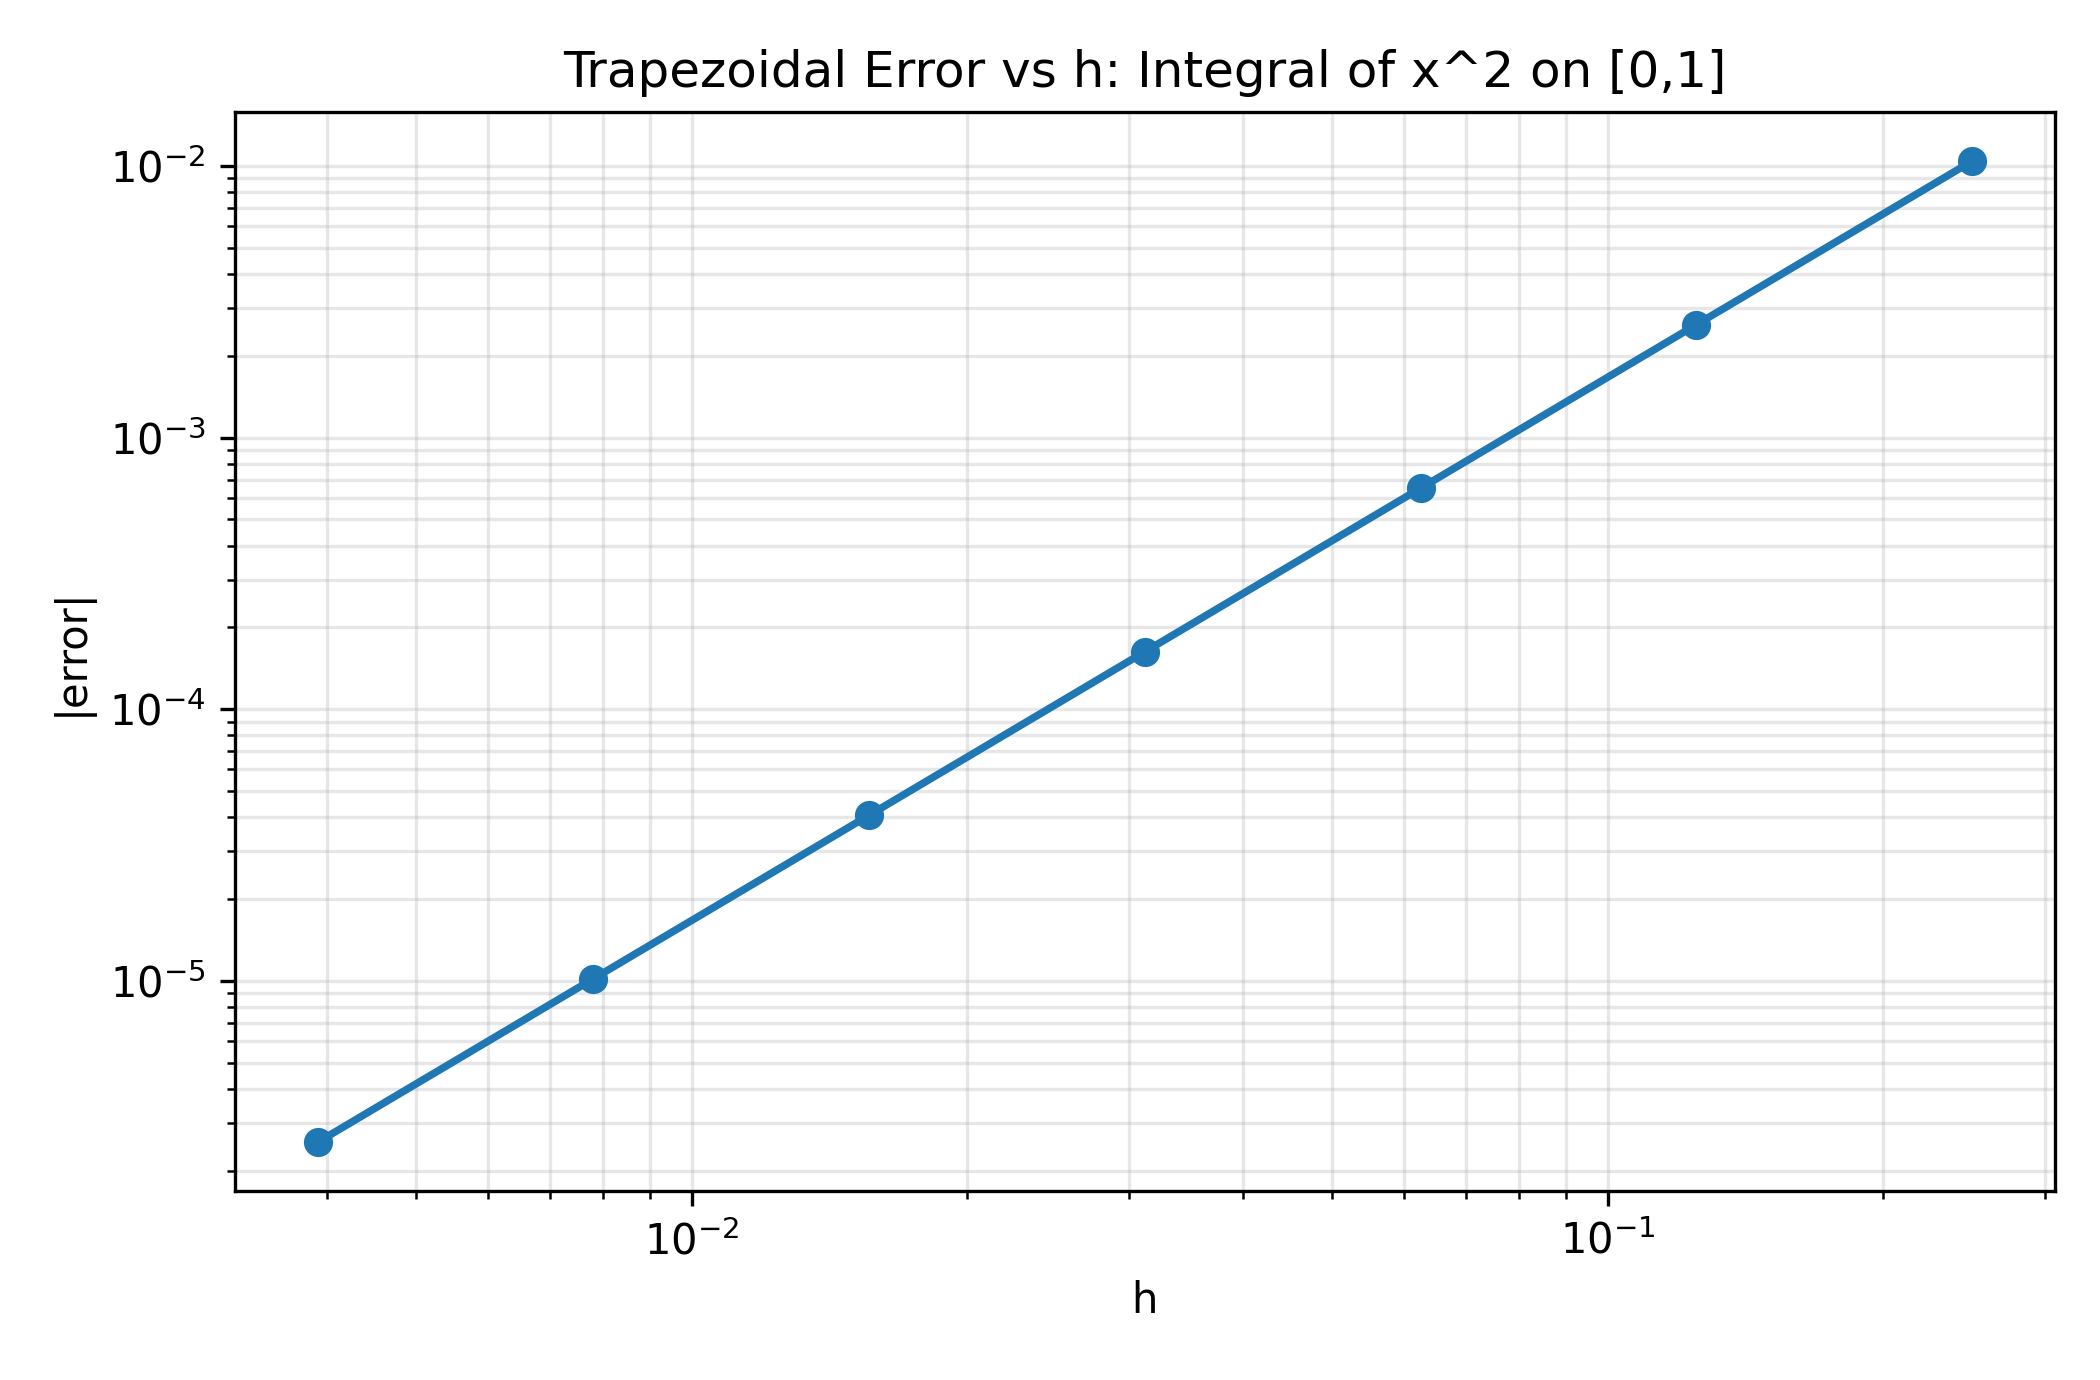
\includegraphics[width=\columnwidth]{../results/plots/integration_trapezoidal_error_vs_h.png}
    \caption{Composite trapezoidal absolute error versus step size $h$ for the $\pi$ benchmark.}
    \label{fig:trap-error}
\end{figure}

\begin{figure}[h!]
    \centering
    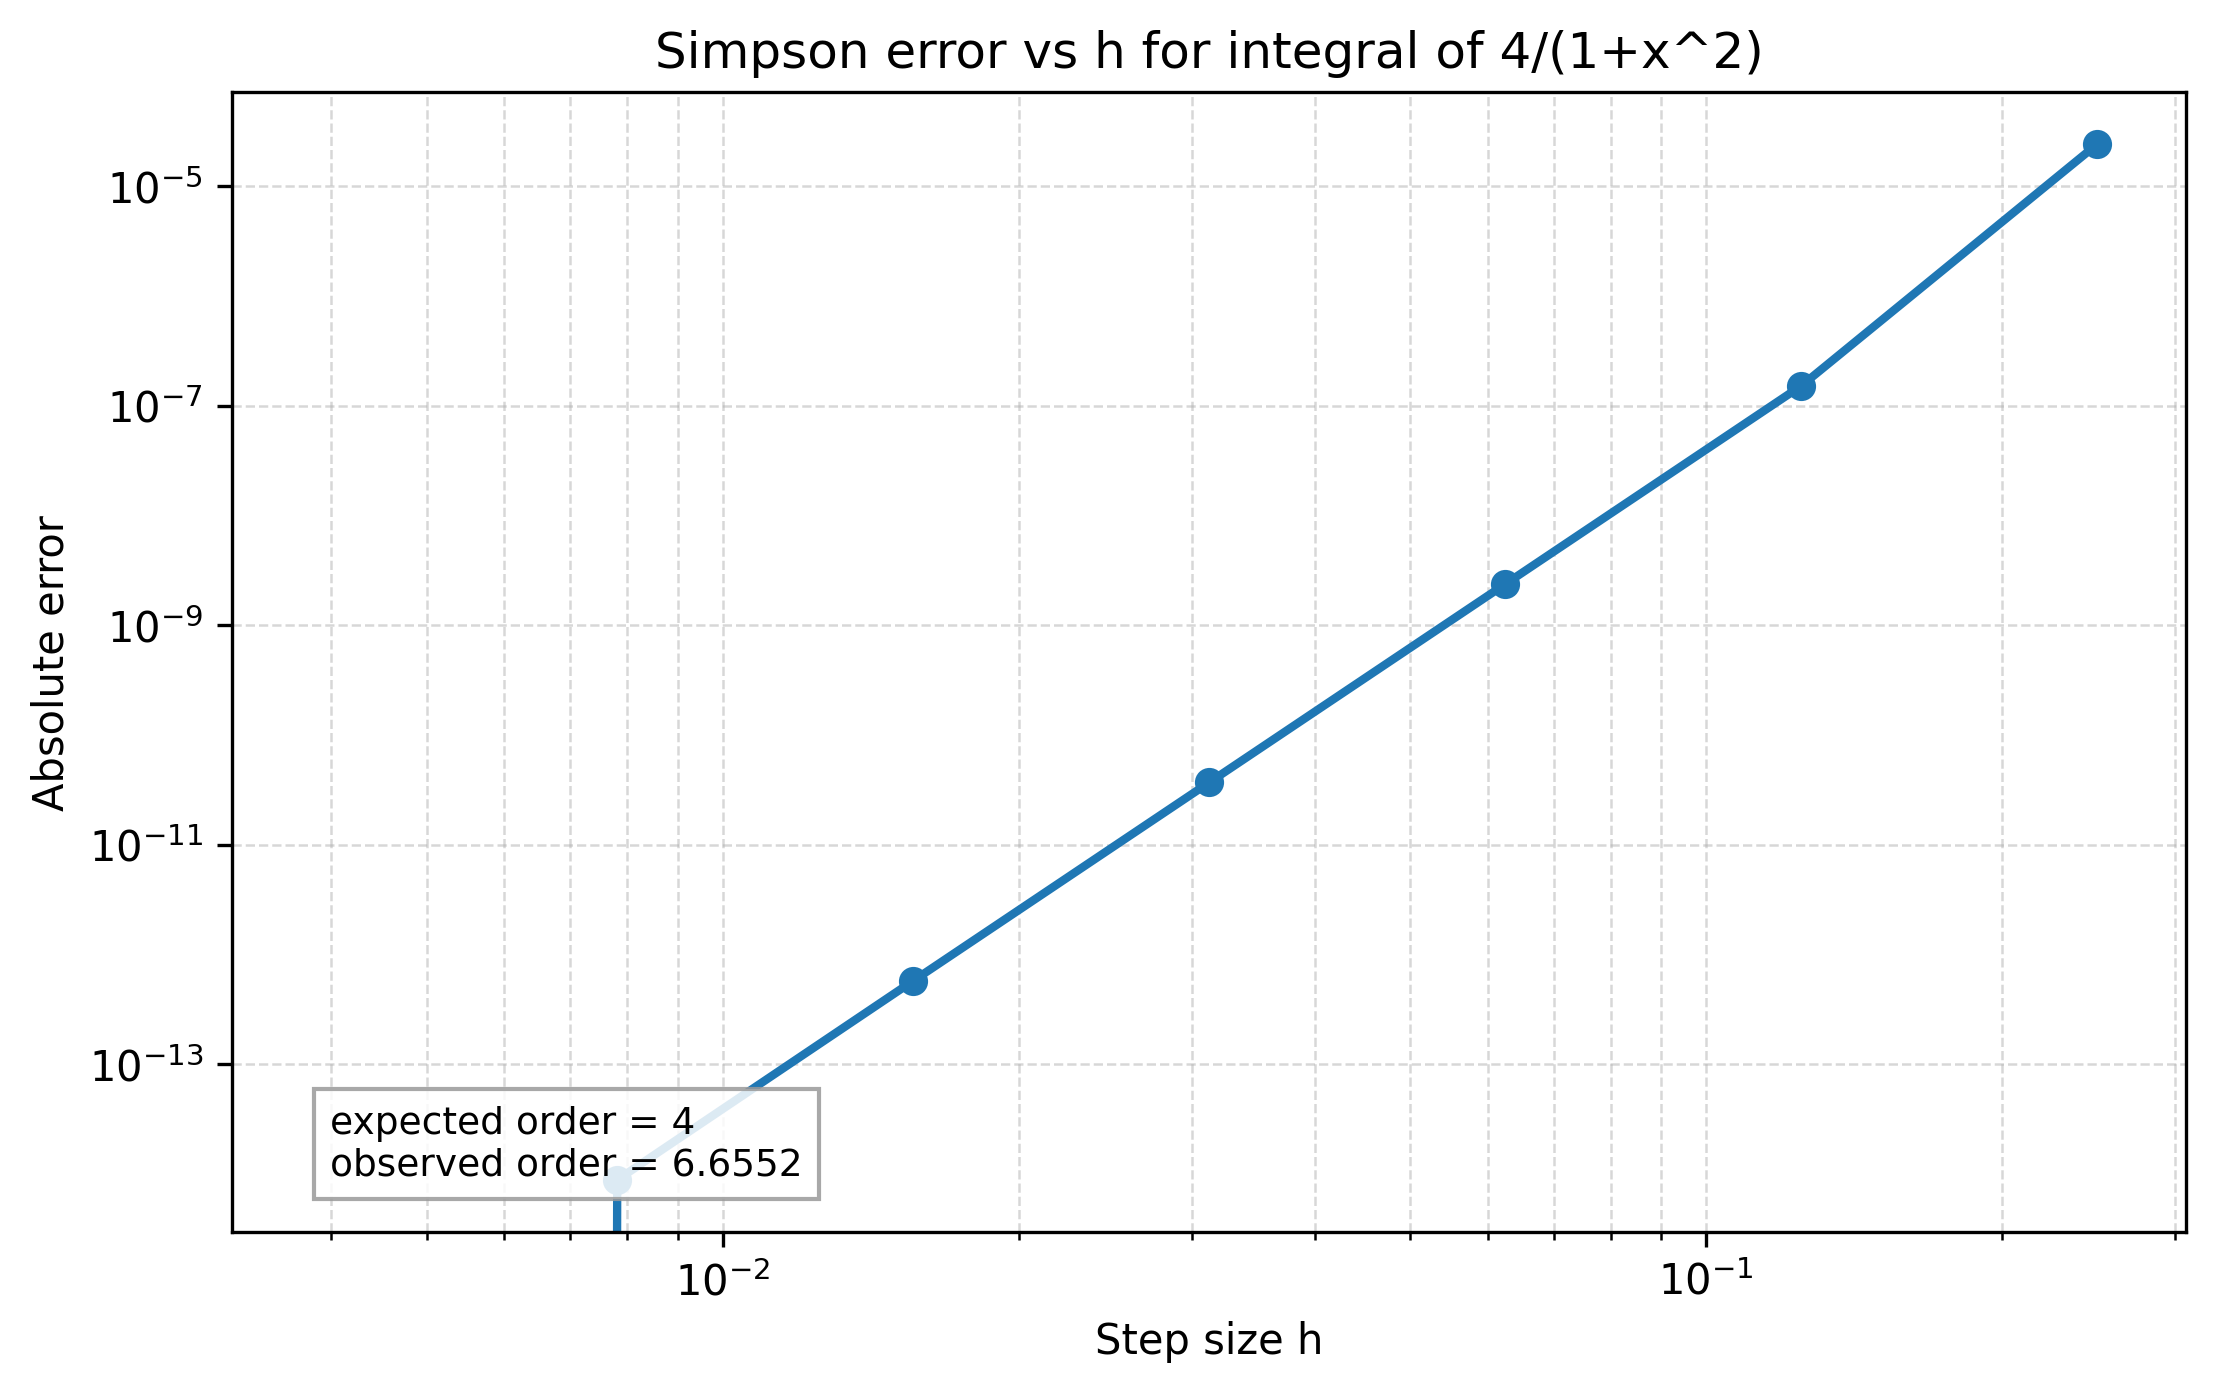
\includegraphics[width=\columnwidth]{../results/plots/integration_simpson_error_vs_h.png}
    \caption{Composite Simpson absolute error versus step size $h$ for the $\pi$ benchmark.}
    \label{fig:simp-error}
\end{figure}

%%%%%%%%%%%%%%%%%%%%%%%%%%%%%%%%%%
% Free-Fall Experiment
%%%%%%%%%%%%%%%%%%%%%%%%%%%%%%%%%%
\section{Free-Fall Experiment}
A drop test recorded the vertical displacement $y$ of a falling object at seven instants. Downward motion is represented by negative displacement (Table~\ref{tab:freefall-data}).

\begin{table}[h!]
\caption{Free-fall position-versus-time measurements}
\vspace{12pt}
\label{tab:freefall-data}
\centering
{\small
\setlength{\tabcolsep}{4pt}
\begin{tabular}{|c|c|c|}
\hline
Index & Time (s) & Position (m) \\\hline
0 & \num{0.000000} & \num{ 0.00} \\\hline
1 & \num{0.100764} & \num{-0.05} \\\hline
2 & \num{0.141736} & \num{-0.10} \\\hline
3 & \num{0.174306} & \num{-0.15} \\\hline
4 & \num{0.201042} & \num{-0.20} \\\hline
5 & \num{0.224583} & \num{-0.25} \\\hline
6 & \num{0.247569} & \num{-0.30} \\\hline
\end{tabular}
}
\end{table}

A degree-2 polynomial $\hat{y}(t) = a_{2}t^{2}+a_{1}t+a_{0}$ is fitted to these data with the coefficients
\[
a_{2} = \num{-4.845194}, \quad a_{1} = \num{-0.019173}, \quad a_{0} = \num{2.593e-4}.
\]
The central three-point formula is applied to $\hat{y}(t)$ at the middle sample time $t_{0}=\qty{0.174306}{s}$. Figure~\ref{fig:freefall} shows the interpolant overlaid on the measured data.

\begin{figure}[h!]
    \centering
    
\includegraphics[width=\columnwidth]{../results/plots/freefall_gravity_interpolation.png}
    \caption{Quadratic interpolant (solid curve) fitted to seven free-fall samples (circles). The evaluation point $t_{0}$ is marked; the title reports the estimated $|\hat{g}|$.}
    \label{fig:freefall}
\end{figure}

%%%%%%%%%%%%%%%%%%%%%%%%%%%%%%%%%%
% Results
%%%%%%%%%%%%%%%%%%%%%%%%%%%%%%%%%%
\section{Results}

\subsection{Analytic Differentiation}
Table~\ref{tab:analytic} lists the absolute error for each method-function combination. All nine cases pass their tolerance.

\begin{table}[h!]
\caption{Analytic differentiation absolute errors ($h=\num{1e-5}$)}
\vspace{12pt}
\label{tab:analytic}
\centering
{\small
\setlength{\tabcolsep}{3pt}
\sisetup{scientific-notation=true,round-mode=figures,round-precision=3}
\begin{tabular}{|l|l|c|c|}
\hline
Function & Method & Abs.\ Error & Pass \\\hline
$\sin(\pi/4)$ & central  & $\num{1.40e-11}$ & Yes \\\hline
              & forward  & $\num{3.04e-11}$ & Yes \\\hline
              & backward & $\num{8.24e-12}$ & Yes \\\hline
$e^{0.3}$     & central  & $\num{2.17e-11}$ & Yes \\\hline
              & forward  & $\num{3.38e-11}$ & Yes \\\hline
              & backward & $\num{8.93e-11}$ & Yes \\\hline
$p'(1.2)$     & central  & $\num{1.26e-10}$ & Yes \\\hline
              & forward  & $\num{1.40e-10}$ & Yes \\\hline
              & backward & $\num{1.40e-10}$ & Yes \\\hline
\end{tabular}
}
\end{table}

Figure~\ref{fig:sine-error} shows how the absolute error varies with step size for the $\sin(x)$ case. The log-log plot confirms $O(h^{2})$ convergence across the mid-range of $h$; floating-point cancellation degrades accuracy below $h\approx\num{1e-6}$.

\begin{figure}[h!]
    \centering
    
\includegraphics[width=\columnwidth]{../results/plots/sine_at_pi_over_4_error_vs_h.png}
    \caption{Absolute error versus step size for $\sin'(\pi/4)$. The $O(h^{2})$ slope is visible in the convergence region.}
    \label{fig:sine-error}
\end{figure}

\subsection{Method Summary}
Table~\ref{tab:summary} summarises performance by method across all three analytic cases.

\begin{table}[h!]
\caption{Per-method error summary over three analytic cases}
\vspace{12pt}
\label{tab:summary}
\centering
{\small
\setlength{\tabcolsep}{3pt}
\sisetup{scientific-notation=true,round-mode=figures,round-precision=3}
\begin{tabular}{|l|c|c|c|}
\hline
Method   & All Pass & Max Abs.\ Err. & Mean Abs.\ Err. \\\hline
central  & Yes & $\num{1.26e-10}$ & $\num{5.39e-11}$ \\\hline
forward  & Yes & $\num{1.40e-10}$ & $\num{6.82e-11}$ \\\hline
backward & Yes & $\num{1.40e-10}$ & $\num{7.93e-11}$ \\\hline
\end{tabular}
}
\end{table}

\subsection{Gravity Estimation}
The second derivative of the quadratic interpolant at $t_{0}=\qty{0.174306}{s}$ yields the signed acceleration
\[
\hat{a} = \qty{-9.6904}{m/s^2},
\]
indicating downward motion consistent with the sign convention. Table~\ref{tab:gravity} compares the estimated magnitude against the standard value.

\begin{table}[h!]
\caption{Free-fall gravity estimation result}
\vspace{12pt}
\label{tab:gravity}
\centering
{\small
\setlength{\tabcolsep}{3pt}
\begin{tabular}{|l|c|}
\hline
Quantity & Value \\\hline
$|\hat{g}|$ (m/s$^{2}$)       & $\num{9.6904}$ \\\hline
Standard $|g|$ (m/s$^{2}$)    & $\num{9.8100}$ \\\hline
Magnitude error (m/s$^{2}$)   & $\num{0.1196}$ \\\hline
Tolerance (m/s$^{2}$)         & $\num{0.1500}$ \\\hline
Pass                           & Yes            \\\hline
\end{tabular}
}
\end{table}

%%%%%%%%%%%%%%%%%%%%%%%%%%%%%%%%%%
% Error Analysis
%%%%%%%%%%%%%%%%%%%%%%%%%%%%%%%%%%
\section{Error Analysis}
For the analytic cases, the central difference consistently achieves the smallest or near-smallest absolute error (Table~\ref{tab:summary}). The maximum error across all methods is $\num{1.40e-10}$, far below the loosest tolerance of $\num{1e-7}$. The log-log error plots confirm $O(h^{2})$ behaviour in the convergence region and the onset of floating-point cancellation at very small $h$.

For integration, trapezoidal errors decrease by roughly a factor of 4 when $h$ is halved, matching second-order convergence. Simpson errors initially decrease much faster and then saturate at floating-point limits; this causes the fitted order to exceed the theoretical value because near-zero terminal errors dominate the regression window.

For the gravity estimate, the primary source of error is the measurement resolution of the position data, which is quantised to the nearest \qty{5}{cm}. The fitted coefficient $a_{2}=\num{-4.845194}$~m/s$^{2}$ implies $2a_{2}=\qty{-9.6904}{m/s^2}$, differing from the accepted $\qty{9.81}{m/s^2}$ by approximately $1.2\%$. This is consistent with the coarse position resolution and indicates that the numerical differentiation step introduces negligible additional error.

%%%%%%%%%%%%%%%%%%%%%%%%%%%%%%%%%%
% Discussion
%%%%%%%%%%%%%%%%%%%%%%%%%%%%%%%%%%
\section{Discussion}
The central formula outperforms both one-sided stencils on every analytic test case, which is expected from its symmetric cancellation of the odd-order Taylor-series error terms. The forward and backward formulas perform comparably to each other and remain within one order of magnitude of the central result---all well within the prescribed tolerances.

The integration benchmark reinforces expected method behavior: trapezoidal is robust and predictably second-order, while Simpson is substantially more accurate for smooth functions at equal mesh densities. For this integrand, Simpson reaches machine-level agreement with $\pi$ at moderate refinement.

The free-fall validation demonstrates that physically meaningful constants can be recovered from a small, coarsely sampled dataset by combining quadratic interpolation with numerical differentiation. Fitting a polynomial first converts the discrete samples into a smooth, differentiable surrogate; double application of the central formula then extracts the acceleration accurately. The $\qty{0.12}{m/s^2}$ discrepancy from the true value of $g$ reflects the position measurement resolution rather than a limitation of the numerical method.

%%%%%%%%%%%%%%%%%%%%%%%%%%%%%%%%%%
% Conclusion
%%%%%%%%%%%%%%%%%%%%%%%%%%%%%%%%%%
\section{Conclusion}
A Python implementation of Unit 03 numerical operators was validated across differentiation and integration tasks. Three-point differentiation passes all analytic checks and supports physically meaningful inference in the free-fall gravity experiment, where $|\hat{g}|=\qty{9.6904}{m/s^2}$ is within tolerance. Composite trapezoidal and Simpson quadrature both satisfy convergence and final-accuracy criteria on the $\pi$ benchmark, with Simpson achieving near machine precision at the finest mesh. Together, these results confirm that the implemented methods are accurate, stable, and suitable for engineering computation on both analytic and measured datasets.

%%%%%%%%%%%%%%%%%%%%%%%%%%%%%%%%%%
% References
%%%%%%%%%%%%%%%%%%%%%%%%%%%%%%%%%%
\small
\begin{thebibliography}{9}
\bibitem{burden}
R. L. Burden and J. D. Faires, \emph{Numerical Analysis}, 10th ed., Cengage Learning, 2015.

\bibitem{chapra}
S. C. Chapra and R. P. Canale, \emph{Numerical Methods for Engineers}, 8th ed., McGraw-Hill, 2020.
\end{thebibliography}

\end{document}
